

\documentclass[conference]{IEEEtran}
\usepackage[utf8]{inputenc} %Codificacion utf-8
\usepackage{graphicx}
\usepackage{amsmath}

\providecommand{\PSforPDF}[1]{#1}



% correct bad hyphenation here
\hyphenation{op-tical net-works semi-conduc-tor}


\begin{document}

\title{Tutorial de trabajo con placa EDU CIAA}

\author{\IEEEauthorblockN{Suarez Facundo,Ezequiel Duperre,Jonathan Saez}
%\author{\IEEEauthorblockN{Ezequiel Duperre}
%\author{\IEEEauthorblockN{Jonathan Saez}
\IEEEauthorblockA{Departamento de Física\\
Universidad Nacional de San Luis\\
San Luis, Argentina\\
Email: fmsuarez92@gmail.com}
}

% make the title area
\maketitle

\IEEEcompsoctitleabstractindextext{%
\begin{abstract}
\boldmath
En este trabajo se pretende desarrollar un tutorial que permita al usuario neófito poder iniciar sus primeros proyectos usando RTOS y comprender la arquitectura de los procesardores Cortex.

\end{abstract}

% Note that keywords are not normally used for peerreview papers.
\begin{IEEEkeywords}
	Cortex M4, Firmware, Makefile, microprocesador,RTOS.
\end{IEEEkeywords}}

\IEEEdisplaynotcompsoctitleabstractindextext

\IEEEpeerreviewmaketitle

\section{Introduction}

% Here we have the typical use of a "T" for an initial drop letter
% and "HIS" in caps to complete the first word.
\IEEEPARstart{P}{ara} el desarrollo de sistemas embebidos es usual iniciarse utilizando placas de pruebas basadas en microcontroladores PIC, sin embargo, el avance del desarrollo de las arquitecturas de los procesadores Cortex, ha llevado a la necesidad del análisis de diversos sistemas embebidos basados en dicho procesador. La placa EDU CIAA nos brinda el ambiente adecuado para la comprensión y para la programación de códigos basados en la arquitectura ARM. 

%	\begin{enumerate}
%		\item \textbf{Accionamientos de velocidad ajustable:} Una aplicación importante de estos accionamientos se encuentra en el control de procesos, donde controlan velocidad de ventiladores, compresores, bombas, sopladores, etc.
%		\item \textbf{Servoaccionamientos:} Por medio de un control avanzado, los motores de inducción se pueden usar como servoaccionamientos en periféricos de computadoras, máquinas herramientas y robótica\cite{Mohan}.
%	\end{enumerate}

\subsection{Descripción de la placa EDU CIAA}
La CIAA es una plaqueta electrónica provista de un microcontrolador y puertos de entrada y salida, cuyo diseño se encuentra disponible en Internet, dicha placa fue concebida para ser utilizada para sistemas de control de procesos productivos, agroindustria, automatización, entre otras; es notable destacar que gracias a la posibilidad del acceso a la información de dicha plataforma, cualquier empresa que desee utilizarla para la elaboración de sus productos puede rediseñarla; de modo que esto fomenta el diseño y la fabricación nacional de sistemas electrónicos.\\



La placa EDU CIAA es la versión educativa de la placa, diseñada con el propósito de conseguir una plataforma base para el desarrollo de proyectos educativos, en este caso, se busca proporcionar las bases del desarrollo de códigos utilizando RTOS.
Sobre la Figura 1 \ref{Fig1} se proporciona el diagrama en bloques de la placa, puede observarse que la placa cuenta con 2 puertos micro-USB (uno para aplicaciones y debugging, otro para alimentación); 4 salidas digitales implementadas con leds RGB, 4 entradas digitales con pulsadores; 1 puerto de comunicaciones RS485 con bornera. La Figura 2 \ref{Fig2} nos muestra  una imagen frontal de la placa; nótese la presencia de dos puertos sobre los cuales se ubican los pines correspondientes a la placa, la Figura 3 \ref{Fig3} ilustra el distribución de dichos pines sobre cada puerto.

%En la Fig. \ref{fig_rotor} se puede observar las características constructivas de un rotor de jaula de ardilla. Y en la Fig. \ref{fig_campos} se pueden observar las velocidades de giro de los flujos magnéticos del rotor y del estator, como así también la velocidad de giro del rotor.

\begin{figure}[!t]
\centering
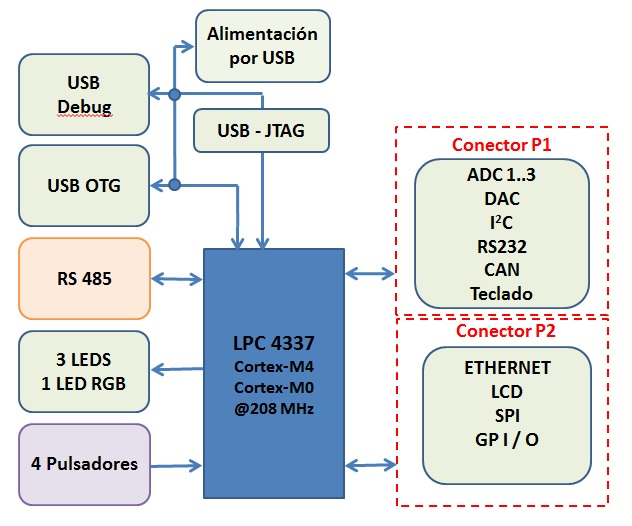
\includegraphics[width=8 cm]{figuras/diagramaenbloques.jpg}
\caption{Diagrama en bloques de EDU CIAA basado en LPC4337.}
\label{Fig1}
\end{figure}

\begin{figure}[!t]
\centering
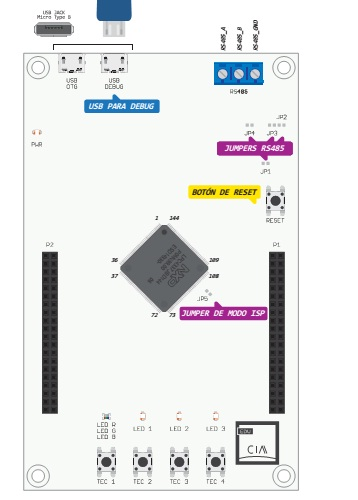
\includegraphics[width=8 cm]{figuras/FIGURA_1.jpg}\\
\caption{Imagen frontal de placa}
\label{Fig2}
\end{figure}

\begin{figure}[!t]
\centering
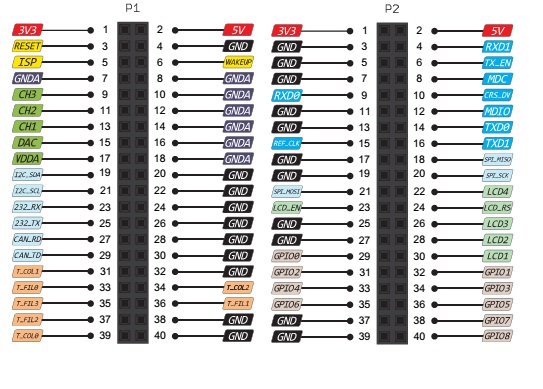
\includegraphics[width=8 cm]{figuras/FIGURA_2.jpg}
\caption{Diagrama de distribucion de los pines sobre la EDU CIAA }
\label{Fig1}
\end{figure}

Sobre el puerto P1, se ubican los siguientes módulos:
\begin{enumerate}
\item 3 entradas analógicas ($ADC0_ 1,2 y 3$)
\item 1 salida analógica (DAC0).
\item 1 puerto I2C.
\item 1 puerto asincrónico full duplex (para RS-232).
\item 1 puerto CAN.
\item 1 conexión para un teclado 3x4.
\end{enumerate}
Sobre el puerto P1, se ubican los siguientes módulos:
\begin{enumerate}
\item 1 puerto Ethernet
\item 1 puerto SPI
\item 1 puerto para Display LCD con 4 bits de datos, Enable y RS.
\item pines genéricos de I/0.
\end{enumerate}

\section{Instalacion de Software}
\subsection{Conceptos previos}
El desarrollo de codigos para sistemas embebidos tiene ciertas semejanzas con el desarrollo de aplicaciones en las PC, en nuestro caso particular se utiliza un compilador llamado \textit{GCC} con soporte para la compilación de proyectos sobre los procesadores basados en la arquitectura ARM, en este caso particular, el compilador utilizado para el procesador de la EDU CIAA (el cual es el LPC4337) se lo denomina \textit{arm-none-eabi-gcc}.\\
Para la ejecución de la depuración de algun programa previamente compilado, el hardware de la CIAA viene provisto con el chip \textit{FT2232H}, que se encarga de hacer un puente entre la interfase JTAG del microcontrolador, y el USB que conecta a la PC en el puerto USB dedicado al debug. Mediante la herramienta de código abierto \textit{OpenOCD (On Chip Debugger)} se controla el chip \textit{FT2232H} por el USB y ademas todo lo referido al JTAG. Luego la herramienta de depuración \textit{GDB} utilizado en el IDE-Eclipse que se instala, se comunica sobre el puerto 3333 (TCP) que el \textit{Open OCD} tiene en escucha esperando la conexión.\\
Debe tenerse en cuenta que el chip \textit{FT2232H} posee 2 canales de comunicación independientes (A y B), sin embargo, ambos salen por el mismo USB, de modo que la PC detecta 2 dispositivos distintos (en realidad es uno compuesto). Uno de ellos, se conecta al JTAG manejado por \textit{OpenOCD} como fue mencionado, mientras que el otro se ve como un puerto virtual COM. Este último sirve principalmente para la depuración.\\
Dado que al fun

\begin{figure}[!t]
\centering
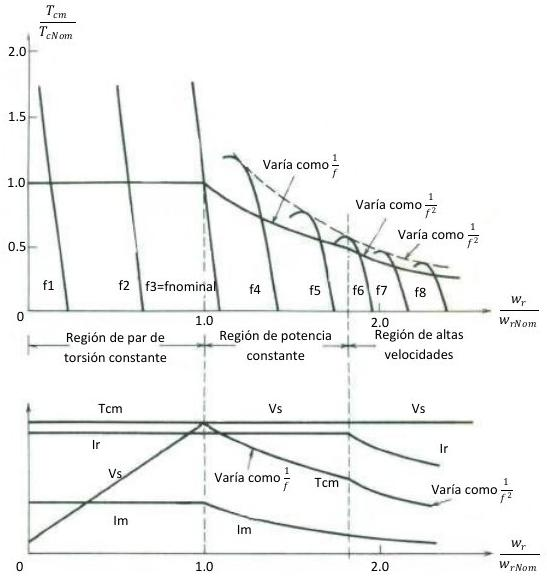
\includegraphics[width=8 cm]{figuras/CurvasMotorInduc.jpeg}\\
\caption{Curvas características del motor de inducción \cite{Mohan}.}
\label{fig_V/F}
\end{figure}

En este trabajo, el sistema de control de velocidad que se ha diseñado trabaja en la zona lineal (región de par de torción constante), es decir, se mantiene constante la relación entre tensión de alimentación y frecuencia de la señal trifásica de alimentación sin sobrepasar los valores nominales. Esto permite mantener el flujo magnético constante sin saturar el núcleo magnético. Una justificación matemática se puede deducir de la ley de Faraday, mostrada en la ecuación (\ref{eq-uno}).

\begin{equation}
v\left( t\right)=-N\dfrac{d\phi}{dt}\label{eq-uno}
\end{equation}

Si se aplica un voltaje 
$v\left(t\right) = V_{m}\sin(\omega t)$ 
al núcleo, el flujo $\phi$ resultante es:

\begin{equation}
\phi (t)=\frac { 1 }{ { N }_{ p } } \int { v(t)dt }= \frac { 1 }{ { N }_{ p } } \int { { V }_{ M }\sin { (\omega t)} dt } 
\end{equation}

\begin{equation}
\phi(t)=-\frac { { V }_{ M } }{ \omega{ N }_{ p } } cos(\omega t)\label{eq-tres}
\end{equation}

La frecuencia eléctrica aparece en el denominador de la ecuación \ref{eq-tres}. Entonces, si se mantiene constante la relación entre la tensión y la frecuencia eléctrica aplicada al estator, el flujo en el núcleo del motor se mantiene constante, al igual que la corriente de magnetización, manteniendo el par motor constante. Esto permite mantener el torque aproximadamente constante entre $0.2*{V}_{nominal}$ y ${V}_{nominal}$. Si se mantiene constante la tensión y se aumenta la frecuencia de alimentación por encima del valor nominal, el torque comienza a disminuir como se observa en la Fig. \ref{fig_V/F}.


\section{Configuración del proyecto}

El proyecto está formado por los distintos módulos que se pueden observar en la Fig. \ref{fig_esq}, los cuales son: DSP, Inversor, Motor Trifásico, Encoder, Bus VCC, Fuente Conmutada Auxiliar y Adaptación de Señales.

\begin{figure}[!t]
\centering
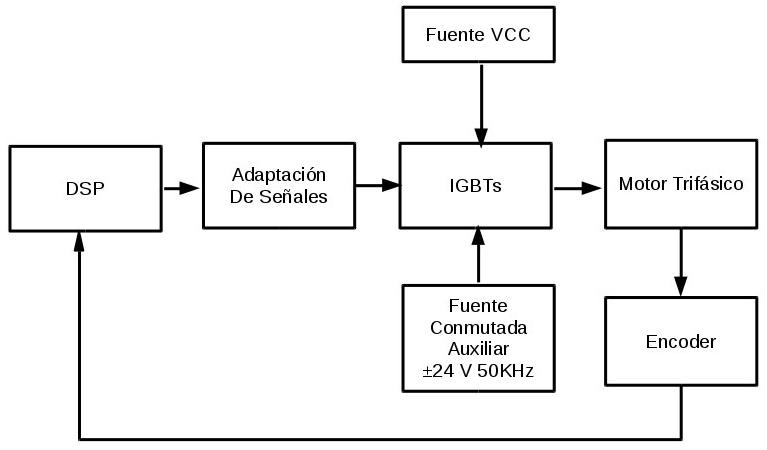
\includegraphics[width=8 cm]{figuras/figura_09.jpeg} \\
\caption{Diagrama esquemático del sistema.} 
\label{fig_esq}
\end{figure}

\subsection{Implementaión del Control V/f en el DSP}

Para la implementación del control V/f se han utilizado las librerías dadas por Texas Instrument a través de su Control Suite \cite{ControlSuite}. Estas librerías permiten un rápido prototipado y puesta a punto del software que se va a cargar en el DSP. En este trabajo en particular se ha utilizado como guía la nota de aplicación \cite{ti} que indica los pasos a seguir para implementar este tipo de control. En la Fig. \ref{fig_bloques} se puede observar un diagrama de bloques con las librerías usadas perteneciente a esta guía. Para la compilación del código se ha usado Code Compose Studio V6 \cite{CCS}.

\begin{figure}[!t]
\centering
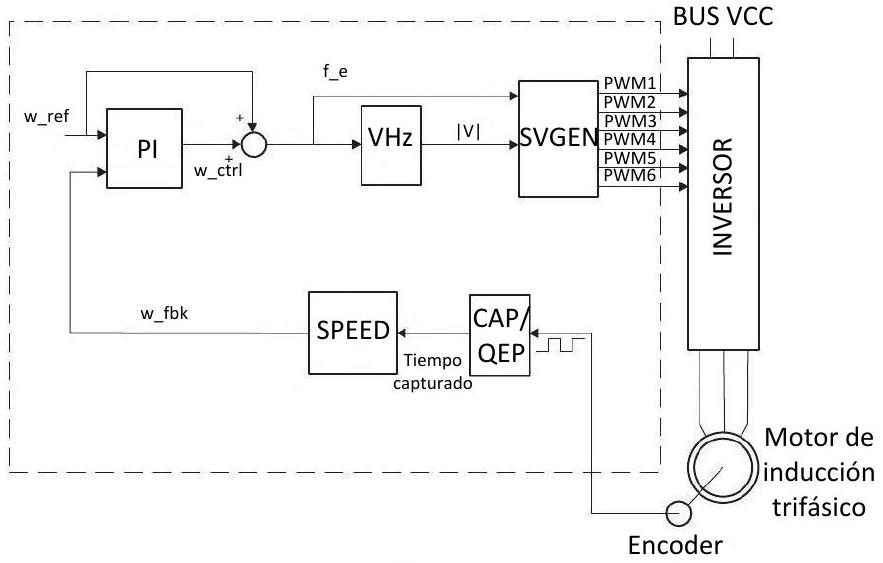
\includegraphics[width=8 cm]{figuras/figura_06.jpeg}\\
\caption{Diagrama de bloques de la implementación del driver para control V/f de un motor de inducción trifásico.} 
\label{fig_bloques}
\end{figure}

Los bloques que están encerrados por la linea punteada de la Fig. \ref{fig_bloques}, corresponden a los bloques software con los cuales se ha programado el DSP. Lo que está fuera de la línea punteada corresponde al inversor, al motor trifásico y al encoder utilizados.

\begin{itemize}
	\item \textbf{Bloque PI:} este bloque define un controlador PI y es el encargado de generar una señal que permita ajustar la velocidad de salida del motor con la velocidad seteada. Esta velocidad se calcula internamente en por unidad (pu).
	\item \textbf{Bloque V/Hz:} Este bloque calcula el módulo de la tensión a aplicar al motor en función del valor de velocidad que recibe.
	\item \textbf{Bloque SVGEN:} Este bloque calcula los coeficientes que son utilizados para generar las señales PWM que generarán las tensiones del estator utilizando la técnica de SVPWM (Space Vector Pulse Width Modulation\cite{Mohan}\cite{Rashid}).
	\item \textbf{Bloque SPEED:} Este bloque calcula la velocidad usando como dato el tiempo capturado por el bloque \textbf{CAP/QEP}.
	\item \textbf{CAP/QEP:} Este bloque está conectado directamente con un módulo hardware del DSP que permite capturar las señales del encoder en forma independiente del procesador.
\end{itemize}


Este sistema trabaja con interrupción de un timer que permite ajustar la frecuencia del PWM, la cual es de 20 KHz. El flujo de ejecución del software es como sigue:\\

\textbf{Dentro del main}
\begin{enumerate}
	\item Se inicializan los módulos software.
	\item Se inicializan las bases de tiempo.
	\item Se habilita la  base de tiempo CNT\_zero de interrupción del EPWM1 y las interrupciones globales.
	\item Se inicializan otros sistemas y parámetros de otros módulos en el caso de que sea necesario.
	\item Se ingresa en un bucle infinito para esperar las interrupciones del EPWM1.
\end{enumerate}


\textbf{Dentro de la interrupción EPWM1}
\begin{enumerate}
	\item Se guarda el contexto y se limpian las banderas de interrupción.
	\item Se ejecuta el módulo PI.
	\item Se ejecuta el módulo V/Hz.
	\item Se ejecuta el módulo SVGEN.
	\item Se ejecuta el módulo CAP/QEP.
	\item Se ejecuta el módulo SPEED.
	\item Se cargan los valores calculados al módulo PWM.
	\item Se restaura el contexto.
	\item Se retorna al bucle infinito.
\end{enumerate}

Los bloques mostrados en la Fig. \ref{fig_bloques} se describe a continuación.



\subsection{Inversor}
Un inversor trifásico es un circuito que convierte corriente contínua (CC) en corriente alterna (CA) de tres fases. Esto se hace mediante la conmutación de dispositivos semiconductores que lo componen, los cuales actúan como llaves. Actualmente son muchas las topologías que se utilizan. En este trabajo se ha utilizado la topología VSI  (\textit{Voltage Source Inverter})\cite{Rashid}, mostrada en la Fig. \ref{fig_esqInv}.

\begin{figure}[!t]
\centering
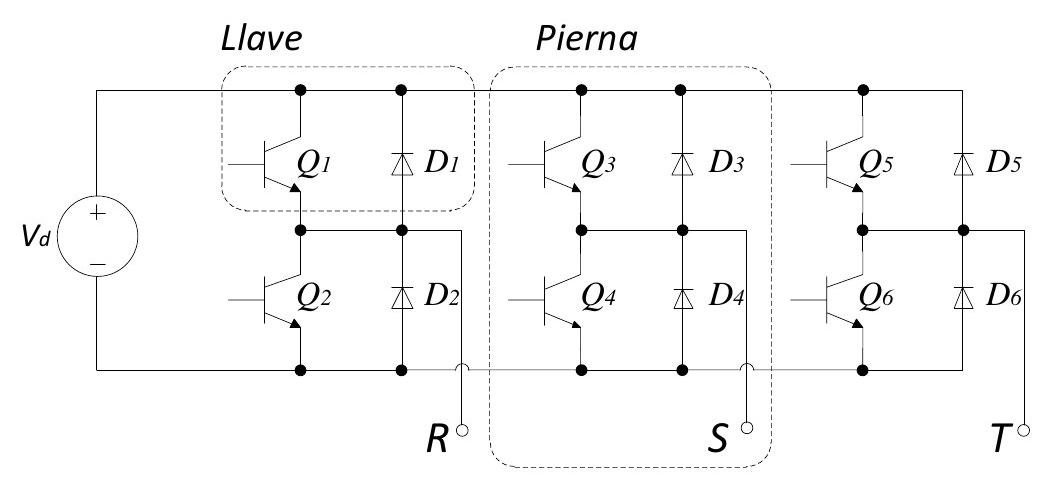
\includegraphics[width=8 cm]{figuras/figura_08.jpeg}
\caption{Diagrama esquemático de un inversor trifásico.} 
\label{fig_esqInv}
\end{figure}

La naturaleza de este circuito impone dos reglas que garantizan su correcto funcionamiento, a saber:

\begin{itemize}
\item Las llaves de una misma pierna no pueden estar cerradas al mismo tiempo, ya que esto produciría un cortocircuito en el bus de CC.
\item Las llaves de una misma pierna no pueden estar abiertas al mismo tiempo, ya que esto dejaría que la tensión en el punto medio de la pierna dependa del sentido de circulación de la corriente por la carga.
\end{itemize}

Las reglas propias de estos sistemas ya están contempladas en las librerías que propone Texas Instrument. En este caso es el bloque \textbf{PWM} de la librería \textbf{\textit{"f2833xpwm.h"}} el que se encarga de que en nigún momento estén cerradas o abiertas al mismo tiempo dos llaves de una misma pierna.

En este trabajo el inversor que se usó se muestra en la Fig. \ref{fig_placaI}, el cual posee un módulo PM25RSK120 marca Mitsubishi, Fig. \ref{fig_PM25R}.

\begin{figure}[!t]
\centering
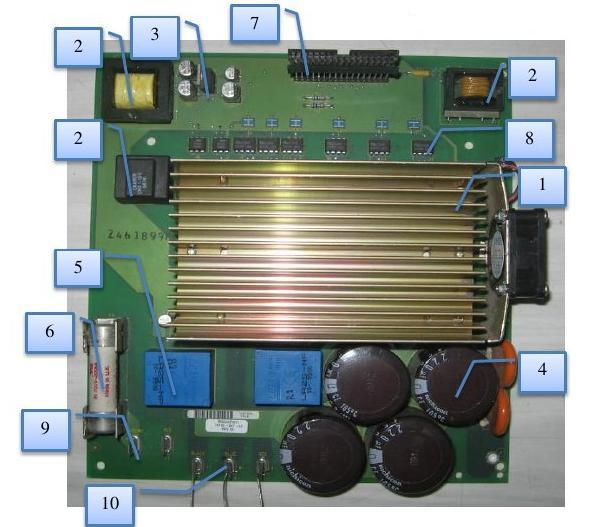
\includegraphics[width=8 cm]{figuras/figura_10.jpeg} \\
\caption{Placa inversora.} 
\label{fig_placaI}
\end{figure}

En la Fig. \ref{fig_placaI} se puede ver el disipador (1), debajo del cual se encuentra el módulo PM25RSK120, sus respectivas fuentes de alimentación (2), una fuente de 5 V (3), filtros del bus de CC (4), circuitos de monitoreo (5), protección (6), conectores para el control de llaves (7), optoacopladores (8), conectores para el bus de CC (9) y para las líneas de salida de la señal trifásica (10). El módulo PM25RSK120, es un módulo inteligente de potencia compuesto por siete llaves IGBT con sus respectivos circuitos de activación y protecciones. 

\begin{figure}[!t]
\centering
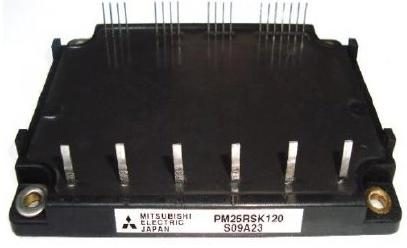
\includegraphics[width=8 cm]{figuras/figura_11.jpeg} 
\caption{Módulo: PM25RSK120, Marca: Mitsubishi.} 
\label{fig_PM25R}
\end{figure}

\subsection{Bus de VCC}

Para el bus  VCC se ha utilizado una fuente doble puesta en serie, la cual entrega una tensión de 60 V y 3 A máximos. Esto permite realizar las pruebas del proyecto sin correr riesgos.

Como el motor utilizado funciona con una tensión trifásica de 380 V y 50 Hz, se tuvo que calcular la nueva frecuencia máxima de trabajo, suponiendo que el motor va a trabajar sin carga. 

En el caso de este trabajo y debido a que el motor trabaja en vacío la frecuencia máxima de alimentación se fijó a 20 Hz.

\subsection{Fuente Auxiliar}

La placa inversora necesita para su funcionamiento una fuente que entregue una tensión de onda cuadrada de $ \pm 24V $ a 50 KHz. 

\subsection{Motor trifásico}

Se utilizó un motor trifásico conectado en estrella modelo TE1BFOXO marca WEG tipo W22 \cite{WEG}, como se observa en la Fig. \ref{fig_motor}. 

\begin{figure}[!t]
\centering
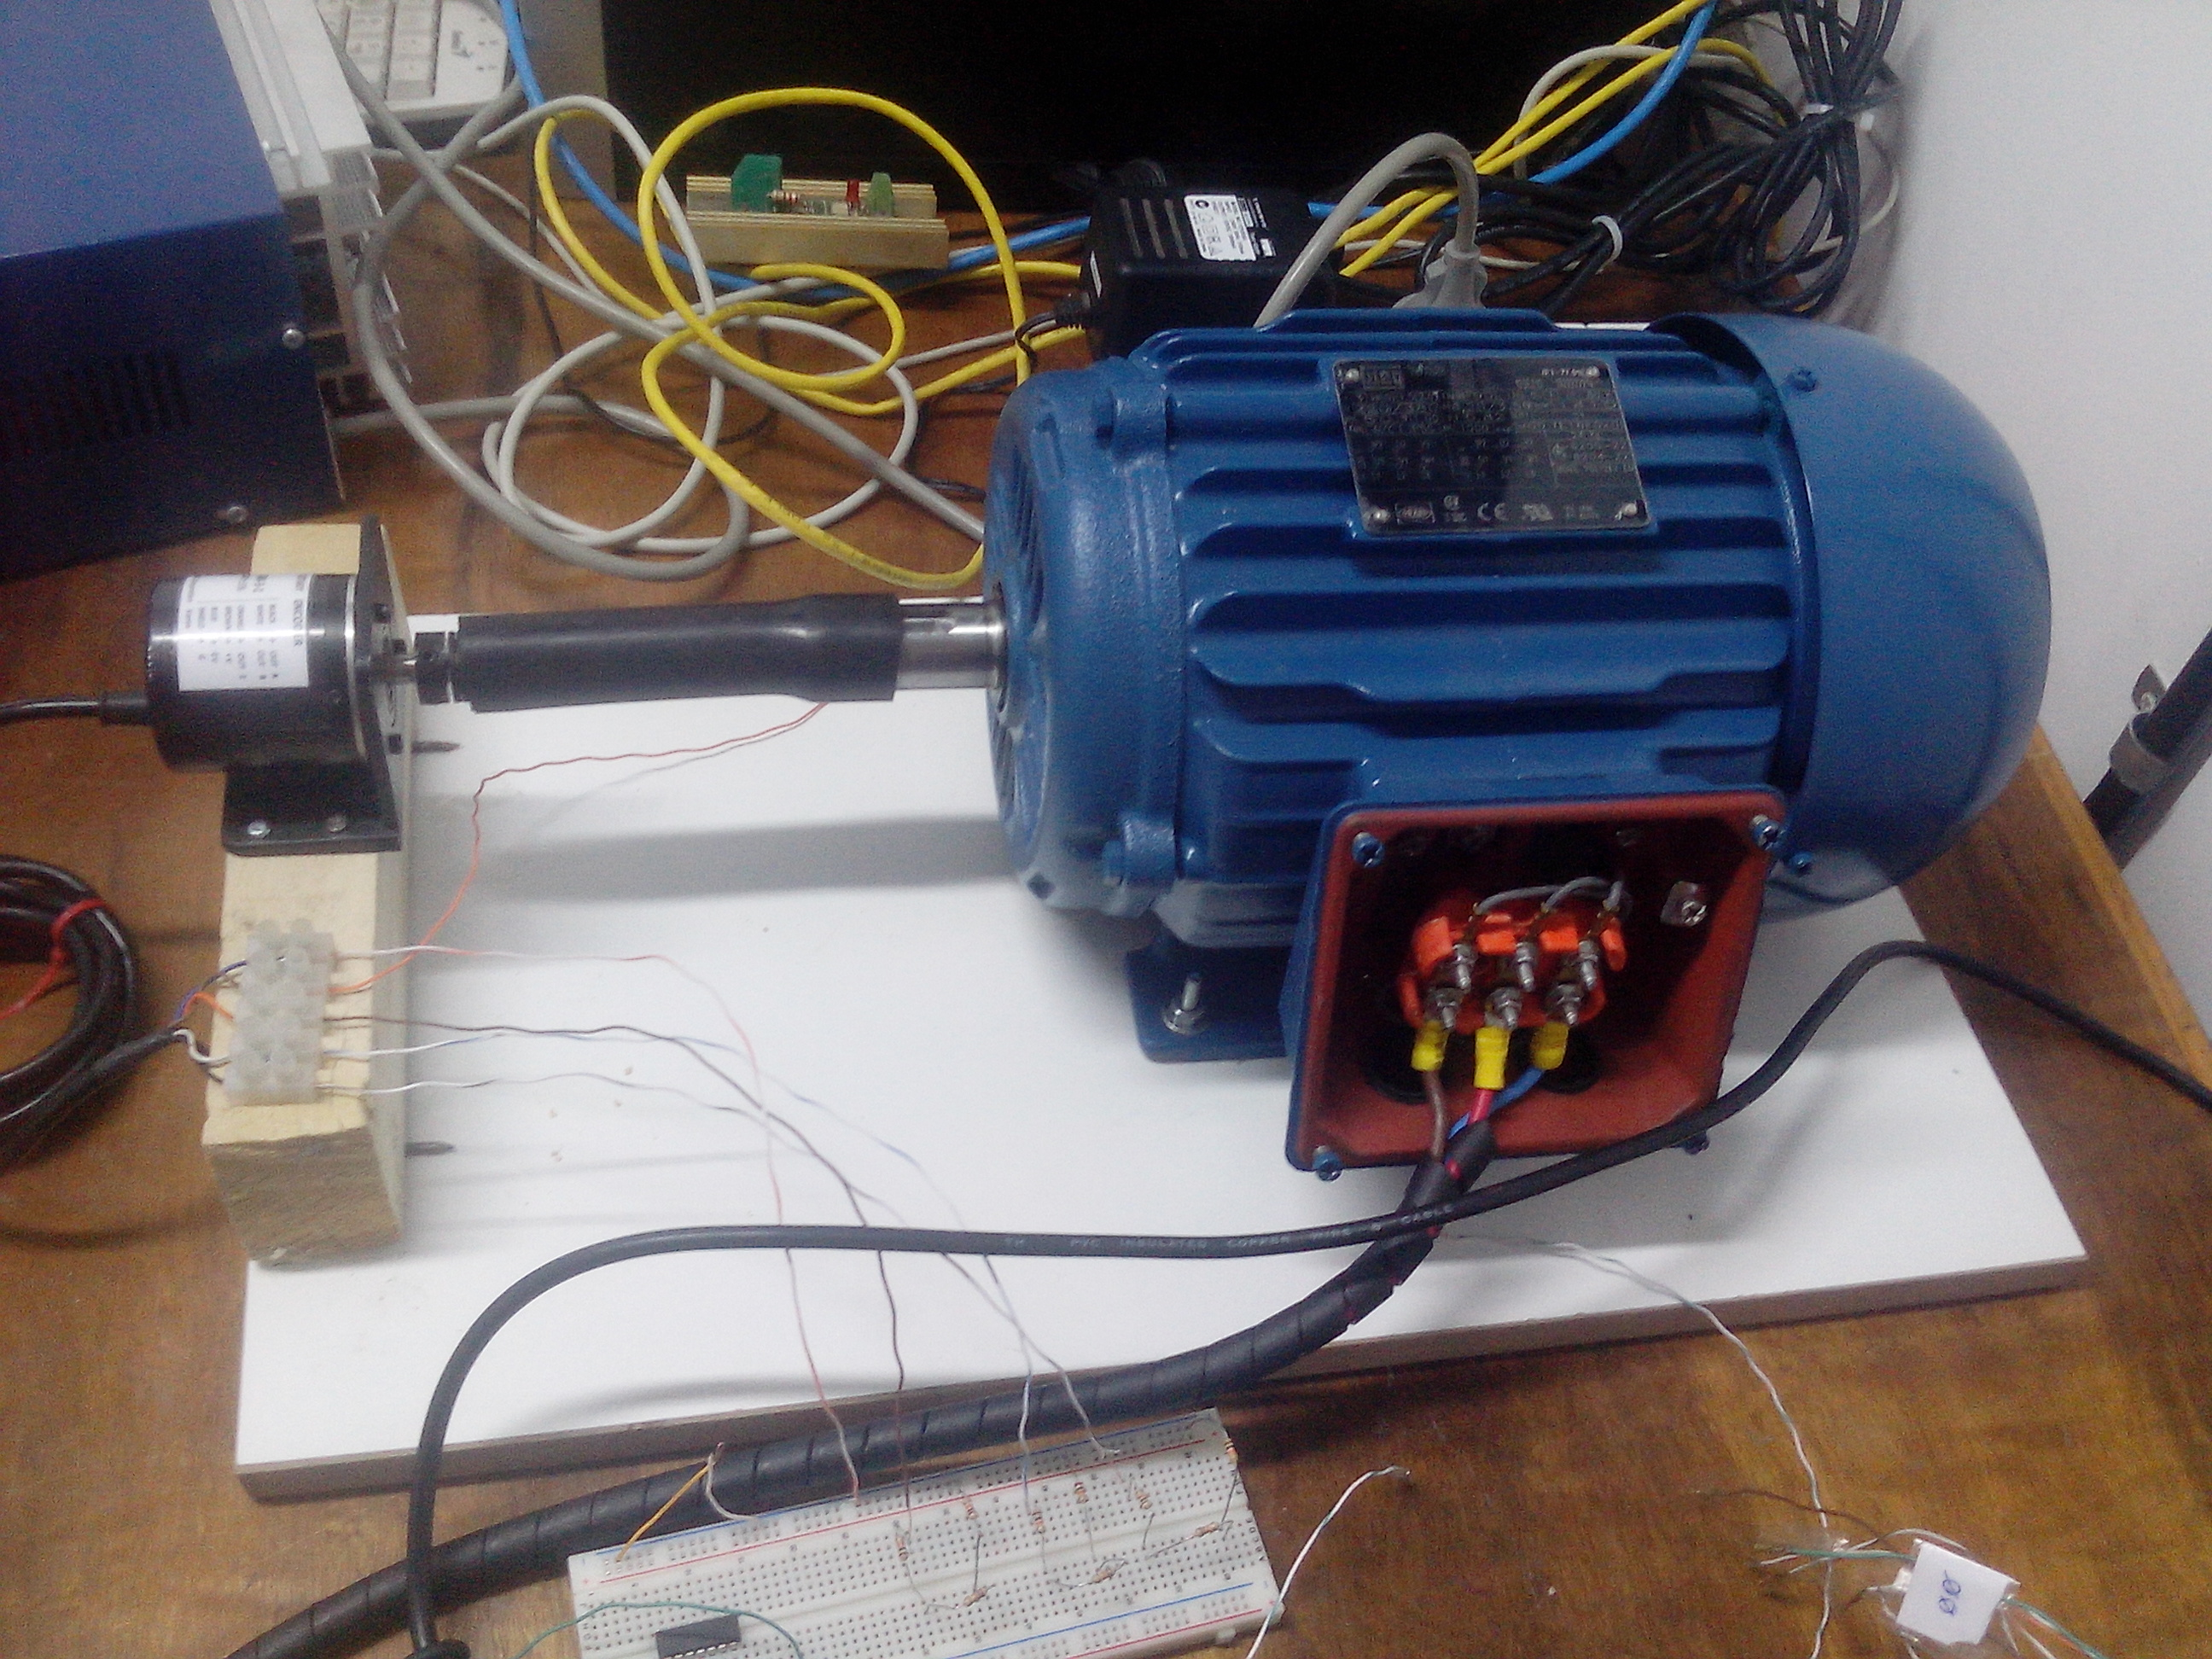
\includegraphics[width=6 cm]{figuras/figura_17.jpeg}\\
\caption{Motor trifásico y encoder acoplado a su eje.}  
\label{fig_motor}
\end{figure}

\subsection{Encoder}

Para medir las RPM desarrolladas por el motor trifásico se ha utilizado un encoder óptico incremental ENB-200-3-1. Este encoder tiene como salida las señales A, B y Z en totem pole, con una resolución de 200 pulsos por revolución.

\section{Pruebas}

Para las pruebas del sistema se usaron las indicaciones de la nota de aplicaciones \cite{ti}. La primera de ella fue probar el código a lazo abierto para ver si las señales PWM correspondían con las esperadas. Se graficó la diferencia entre las señales Ta, Tb y Tc que entran al bloque pwm. El resultado que se obtuvo se muestra en la Fig. \ref{fig_TaTb03}

\begin{figure}[!t]
\centering
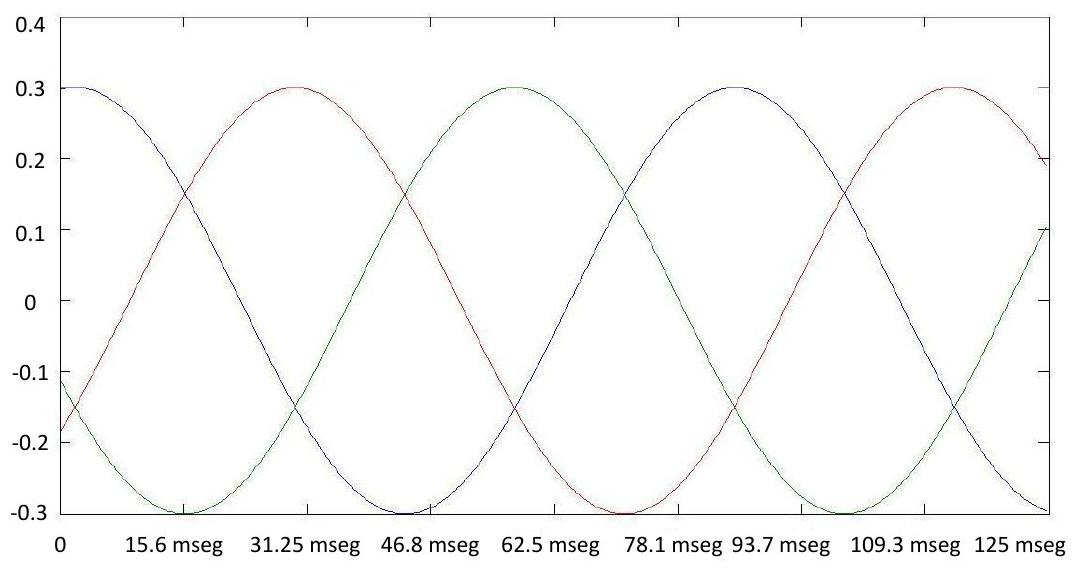
\includegraphics[width=8 cm]{figuras/figura_19.jpeg}\\
\caption{Señales Ta-Tb, Tb-Tc y Tc-Ta al 30\% de la tensión nominal}  
\label{fig_TaTb03}
\end{figure}

En la Fig. \ref{fig_TaTb03} se puede observar que para una tensión $ 0.3*V_{nom} $ la frecuencia es un 30\% de la frecuencia nominal. En el caso de la Fig. \ref{fig_TaTb} la tensión aplicada es la nominal, por lo tanto la frecuencia es la nominal. Con esto queda demostrado que el sistema cumple con los requerimientos.

\begin{figure}[!t]
\centering
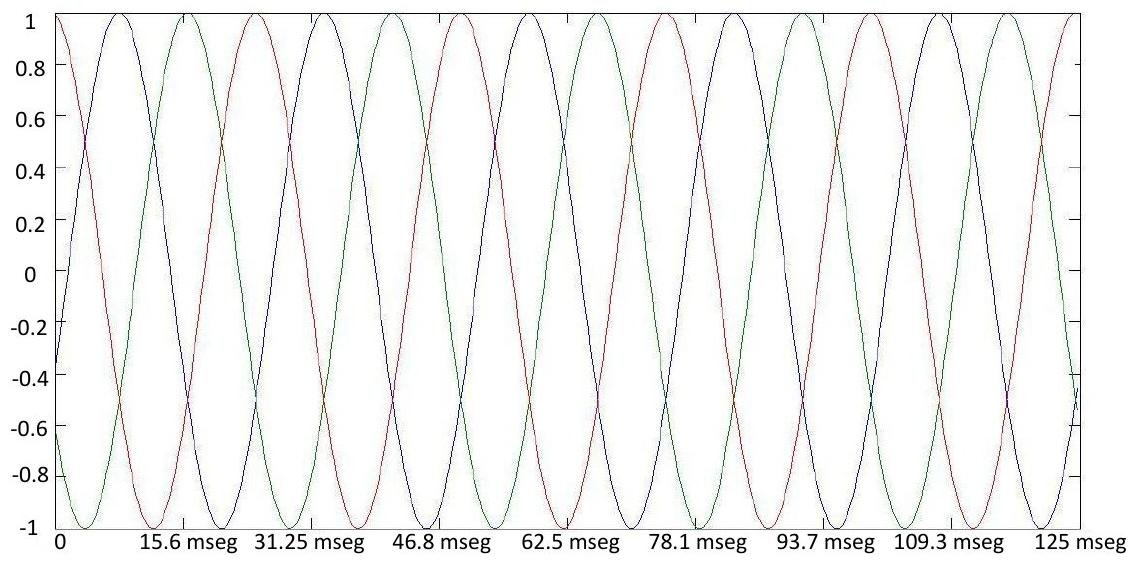
\includegraphics[width=8 cm]{figuras/figura_20.jpeg} \\
\caption{Señales Ta-Tb, Tb-Tc y Tc-Ta a la tensión nominal}
\label{fig_TaTb}
\end{figure}


\subsection{Ajuste del controlador PI}

El módulo PI responde a la ecuación \ref{eq-cuatro}

\begin{equation}
u(t)=K_pe(t)+K_i\int_0^te(\tau)d\tau  \label{eq-cuatro}
\end{equation}


en donde 
\begin{itemize}
	\item u(t) es la salida del PID
	\item e(t) es el error entre la referencia y la retroalimentación
	\item  $ K_p $ es la ganancia proporcional del PID
	\item $ K_i $ es la ganancia integral del PID
\end{itemize}

El módulo PI se ha configurado siguiendo los siguientes pasos:\\
\textbf{Paso 1.}\\
Establecer la ganancia integral $ K_i = 0 $  y la ganancia proporcional $ K_p = 1 $.\\
\textbf{Paso 2.}\\
Mientras se le inyecta una señal escalón a la entrada, ajustar poco a poco  la variable de ganancia proporcional $ K_p $, hasta alcanzar alcanzar el tiempo de subida y overshoot óptimos.\\
\textbf{Paso 3.}\\
Si es necesario, aumentar gradualmente la ganancia integral $ K_i $ para optimizar el retorno de la salida de estado estacionario a nominal. El controlador será muy sensible a este término y se puede volver inestable así que se debe asegurar de comenzar con un número muy pequeño. La ganancia integral se traducirá en un aumento de sobreimpulso y de oscilación, por lo que puede ser necesario disminuir ligeramente el término $ K_p $ de nuevo para encontrar el mejor equilibrio. 


\subsection{Pruebas finales}

Para la prueba del sistema se desarrolló una señal tipo escalón que variaba entre 0.3 y 1. Esta señal tiene un período de 5 segundos. Los resultados se muestran en las Fig. \ref{fig_entEsc}, \ref{fig_salPI_des} y \ref{fig_salPI_asc}.

\begin{figure}[!t]
\centering
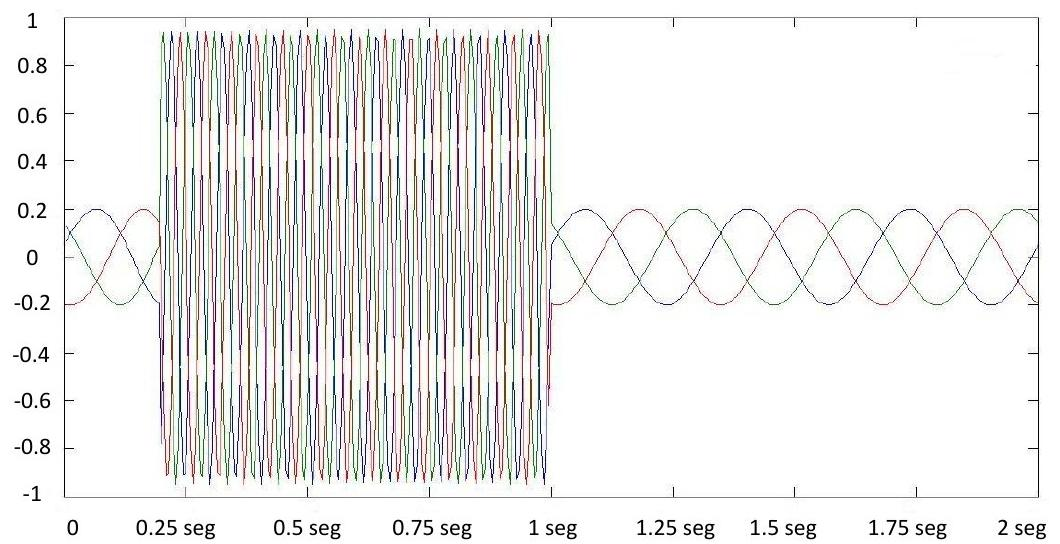
\includegraphics[width=8 cm]{figuras/figura_21.jpeg} \\
\caption{Señales Ta-Tb, Tb-Tc y Tc-Ta dada una entrada escalón} 
\label{fig_entEsc}
\end{figure}
 

\begin{figure}[!t]
\centering
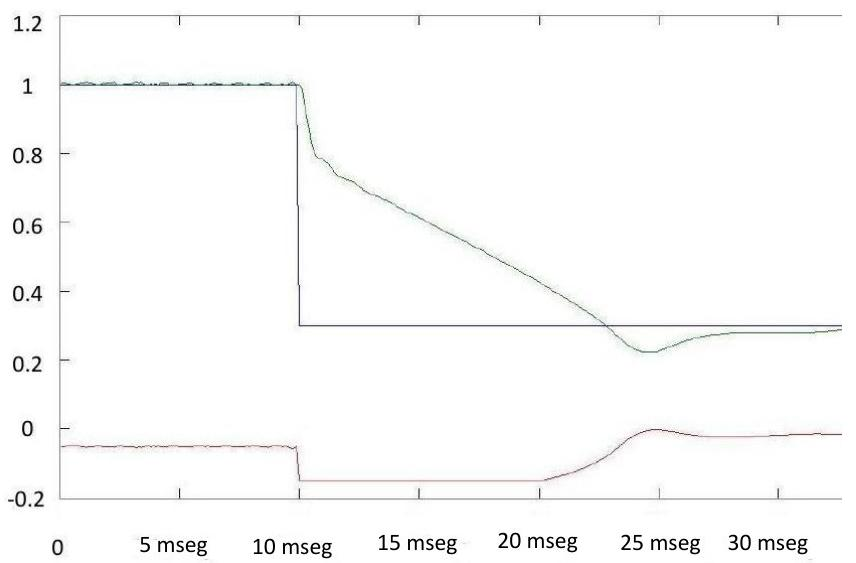
\includegraphics[width=8 cm]{figuras/figura_22.jpeg} \\
\caption{Velocidad, salida del controlador y señal escalón cuando el escalón es descendente} 
\label{fig_salPI_des}
\end{figure}


\begin{figure}[!t]
\centering
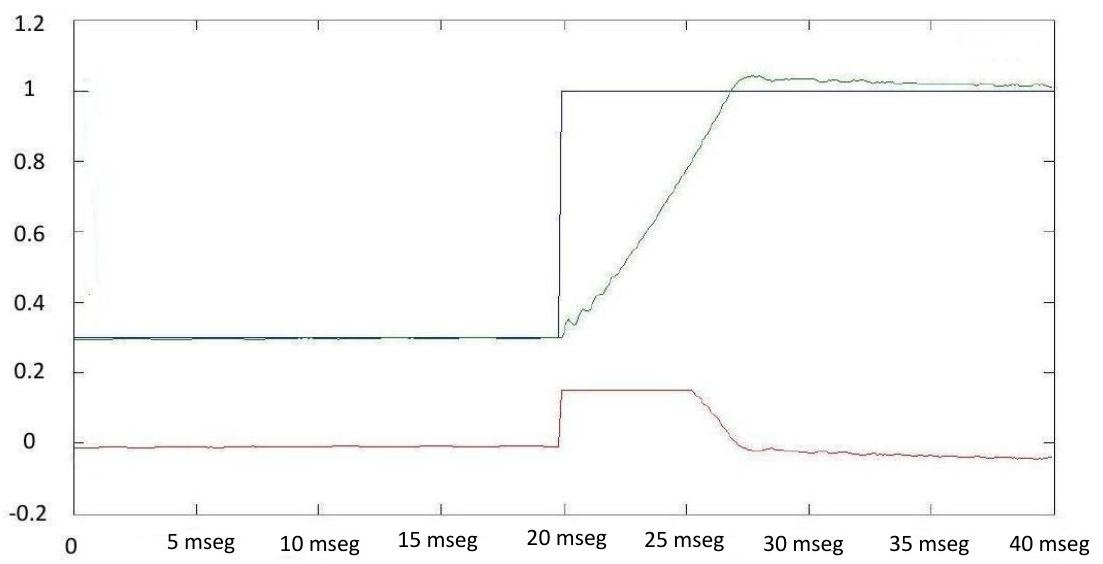
\includegraphics[width=8 cm]{figuras/figura_23.jpeg} \\
\caption{Velocidad, salida del controlador PI y señal escalón cuando el escalón es ascendente} 
\label{fig_salPI_asc}
\end{figure}

\section{Conclusiones}

En este trabajo se ha logrado realizar un contro V/f usando las librerías propias de Texas Instrument. Se logró modificar las librerías y acondicionarlas para el \textbf{DSP TMS320F28335}. Este DSP puede trabajar directamente con datos tipo float, lo cual permitió modificar las librerías y pasarlas a float.
En las pruebas realizadas también se aumentó la carga aplicada al eje del motor y se comprobó que el sistema buscaba ajustar la velocidad de acuerdo con la velocidad de referencia.
También se frenó el motor hasta pararlo, y este volvía a su estado de régimen a la velocidad de referencia.


%\section{Agradeciemientos}



% Can use something like this to put references on a page
% by themselves when using endfloat and the captionsoff option.
\ifCLASSOPTIONcaptionsoff
  \newpage
\fi

\begin{thebibliography}{1}

\bibitem{Mohan} Ned Mohan, Tore M. Undeland, William P Robbins. \textit{Electrónica de Potencia. Convertidores, aplicaciones y diseño.} McGraw Hill. Tercera Edición
\bibitem{Rashid} Muhammad Rashid. \textit{Electróncia de Potencia. Circuitos, dispositivos y aplicaciones.} Pearson Prentice Hall. Tercera Edición.
\bibitem{Alfonso} Alfonso Álzate, Duberney Murillo Yarce, Marcela González Valencia. "Control de velocidad mediante relación voltaje-frecuencia".  ISSN 0122-1701
\bibitem{ControlSuite} http://www.ti.com/tool/controlsuite
\bibitem{ti} Scalar (V/f) Control of 3-Phase Induction Motors. Application Report. http://www.ti.com/lit/an/sprabq8/sprabq8.pdf
\bibitem{DSP} http://www.ti.com/product/TMS320F28335
\bibitem{CCS} Code Composer Studio\\ http://www.ti.com/tool/ccstudio
\bibitem{WEG} http://www.weg.net/w22/index-es.php?market=am-latina

\end{thebibliography}


\end{document}


